\documentclass[letterpaper, 10 pt, conference]{ieeeconf}  
\IEEEoverridecommandlockouts                              
\overrideIEEEmargins                                      

\usepackage{amsmath} 
\usepackage{amssymb} 
\usepackage{graphicx} 

\graphicspath{{./Images/}}

\title{\LARGE \bf Gaussian Process Latent Space Policies for \\ Data-efficient Learning of Robotic Clothing Assistance}

\author{Nishanth Koganti$^{1}$, Tomohiro Shibata$^{2}$, Tomoya Tamei$^{3}$, and Kazushi Ikeda$^{1}$% 
\thanks{$^{1}$Nishanth Koganti and Kazushi Ikeda are with Nara Institute of Science and Technology, Ikoma, Japan
        {\tt\small \{nishanth-k,kazushi\}@is.naist.jp}}%
\thanks{$^{2}$Tomohiro Shibata is with Kyushu Institute of Science and Technology, Kitakyushu, Japan
        {\tt\small tom@brain.kyutech.ac.jp}}%
\thanks{$^{3}$Tomoya Tamei is with Kobe University, Kobe, Japan
        {\tt\small tomo-tam@port.kobe-u.ac.jp}}%
}

\begin{document}

\maketitle
\thispagestyle{empty}
\pagestyle{empty}

\section{Introduction}
Motor-skill learning in robotics is challenging due to high task variability. Robotic assistance to clothing is one such application where the robot needs to interact with non-rigid clothing articles and with the assisted person whose posture can vary. Existing methods in reinforcement learning can be sample-inefficient making it impractical for such applications. Recently, there have been several studies that propose the use of latent variable models to perform data-efficient reinforcement learning~\cite{lrl1, lrl2}. In this study, we propose the use of Bayesian Gaussian Process Latent Variable Model (BGPLVM)~\cite{bgplvm} to learn a low-dimensional representation of motor-skills for robotic clothing assistance in extension to our previous work~\cite{koganti2016}. We implement our framework in a practical setting with a dual-arm robot performing clothing assistance tasks.

\section{Methods}
BGPLVM is a dimensionality reduction technique proposed by Titsias et al.~\cite{bgplvm} derived from the probabilistic model where high-dimensional observations are assumed to be generated from latent inputs through a noisy process,
\begin{equation}
	y = f(x) + \epsilon, \epsilon \sim \mathcal{N}(0,\sigma^2I)
\end{equation}
The mapping function, f, is modeled using a Gaussian Process (GP) leading to data-efficient and non-linear dimensionality reduction. The dimensionality of the latent space can be automatically inferred by using an ARD kernel function in the GP mapping.

In our framework, the latent space learnt with BGPLVM is used in two different ways as shown in Fig.~\ref{figure:overview} i.e.: a) a real-time controller that can be used as a tool for learning from demonstration to impart novel skills to the dual-arm robot and b) to perform policy search reinforcement learning with the BGPLVM latent space as a low-dimensional search space. The representation used for the robot trajectory affects the generalizability of the latent space. We consider two alternate representations i.e. a kinematic representation ($\mathcal{K}$) given by joint angles of 6 DoF dual-arm robot $y_{\mathcal{K}} \in \mathbb{R}^{12}$ and a dynamic representation ($\mathcal{D}$) that also includes the joint angular velocities $y_{\mathcal{D}} \in \mathbb{R}^{24}$.

\begin{figure}
	\centering
	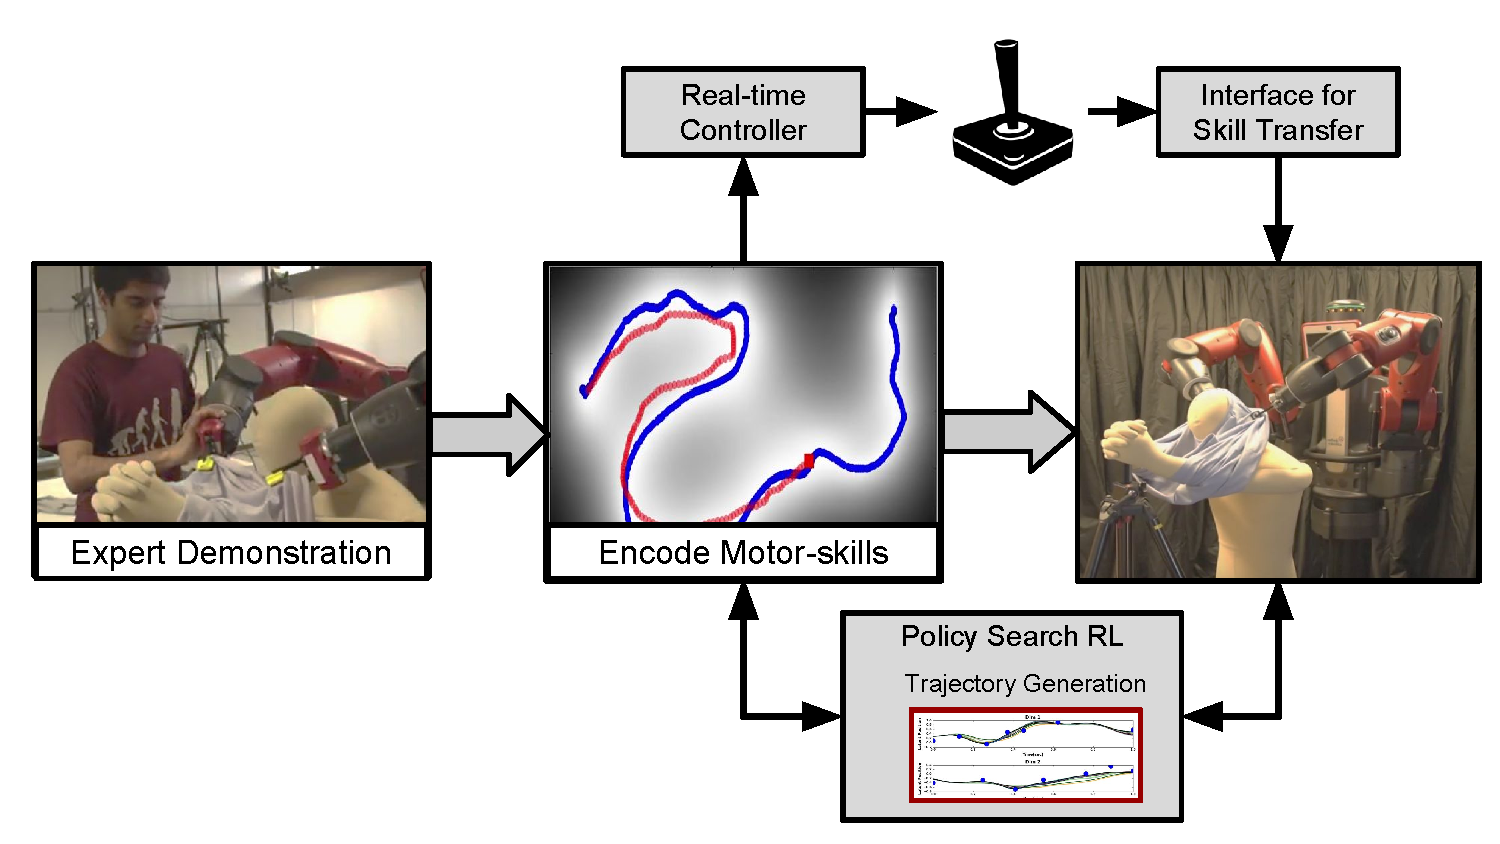
\includegraphics[width=0.4\textwidth]{overview.pdf}
	\caption{Overview of framework using BGPLVM latent space}
	\label{figure:overview}
\end{figure}

\section{Results and Discussion}
In this section, we present the performance of our proposed framework in a practical setting of robotic clothing assistance. The experimental setup includes Baxter research robot, a soft mannequin as the subject and a T-shirt as the clothing article. 
\begin{table}[h]
	\centering
	\caption{Reconstruction Error given by Normalized RMSE}
	\begin{tabular}{|c|c|c|c|}
		\hline
		Input & PCA & GPLVM & BGPLVM \\
		\hline
		$\mathcal{K}$ & 0.040 & 0.054 & \textbf{0.033} \\
		$\mathcal{D}$ & 0.095 & 0.128 & \textbf{0.082} \\
		\hline
	\end{tabular}
	\label{table:results}
\end{table}
Table~\ref{table:results} compares the mean RMSE error of reconstructing high-dimensional robot trajectories from the latent space evalauted using leave-one-out cross validation. The performance is compared with other latent variable models such as PCA and GPLVM. BGPLVM has the best performance irrespective of the representation indicating its generalizability to different trajectories. Models were trained with initial dimensionality as 10 and the ARD kernel selects 2 dimensions as sufficient to model the task. Our future work will be to perform comprehensive analysis and comparison especially in terms of data-efficiency with recent advances in deep reinforcement learning.

\begin{thebibliography}{10}
\bibitem{lrl1}
Sæmundsson, Steindór, et al. ``Meta Reinforcement Learning with Latent Variable Gaussian Processes.'' arXiv preprint arXiv:1803.07551 (2018).
\bibitem{lrl2}
Haarnoja, Tuomas, et al. ``Latent Space Policies for Hierarchical Reinforcement Learning.'' arXiv preprint arXiv:1804.02808 (2018).
\bibitem{bgplvm}
Titsias, Michalis, and Neil D. Lawrence. ``Bayesian Gaussian process latent variable model.'' Proceedings of the Thirteenth International Conference on Artificial Intelligence and Statistics. AISTATS 2010.
\bibitem{koganti2016}
Koganti, Nishanth, et al. ``Bayesian Nonparametric Motor-skill Representations for Efficient Learning of Robotic Clothing Assistance.'' Workshop on Practical Bayesian Nonparametrics, Neural Information Processing Systems. NIPS 2016.
\end{thebibliography}

\end{document}
